\documentclass[a4paper,twoside]{article}

\usepackage[utf8]{inputenc}
\usepackage[ngerman]{babel}

\usepackage{epsfig}
\usepackage{subfigure}
\usepackage{calc}
\usepackage{amssymb}
\usepackage{amstext}
\usepackage{amsmath}
\usepackage{amsthm}
\usepackage{multicol}
\usepackage{pslatex}
\usepackage{apalike}
\usepackage{enumitem}
\usepackage{MOSI}     % Please add other packages that you may need BEFORE the MOSI.sty package.

\newcommand{\team}{Jannik Simon Münz, Ruedi Lüthi}
\newcommand{\theme}{Ausbeutung von Tierpopulationen}
\setcounter{page}{1}

\subfigtopskip=0pt
\subfigcapskip=0pt
\subfigbottomskip=0pt

\begin{document}

	\title{Ausbeutung von Tierpopulationen\subtitle{Wachstumsgleichungen im Vergleich zu einer\\agentenbasierten Modulation und einem zellulären Automaten} }
	
	\author{\authorname{Jannik Simon Münz und Ruedi Lüthi}}
	
	\keywords{Wachstum, Räuber und Beute, agentenbasierte Modellierung, Zellulärer Automat, WATOR}

	\abstract{In dem nachfolgenden Bericht wird die konkrete Implementation einer agentenbasierten Modellierung sowie die eines zellulären Automaten beschrieben. Dabei werden die Resultate der beiden Modelle mit dem klassischen Räuber-Beute Modell verglichen. Dabei konnte beim Betrachten aller Modelle jeweils immer ein Schwingungsverhalten beobachtet werden.}
	
	\onecolumn \maketitle \normalsize \vfill

	\section{\uppercase{Die Wachstumsgleichung}}\label{sec:Wachstumsgleichung}

	\noindent Nachfolgend wird das Wachstum einer Blauwalpopulation als Funktion abhängig von der Zeit \(y(t)\) beschrieben. Ohne äußere Einflüsse wächst die Population der Blauwale um einen konstanten Faktor \(r\) an, wobei das Maximum der Population durch die Umweltkapazität \(K\) begrenzt ist. Von Interesse ist hierbei die Veränderung der Population im Zeitintervall \(\Delta t\). Dies führt zu der folgenden Differentialgleichung:
	\begin{align*}
		y(t+\Delta t) &= y(t) + r\cdot\left(1-\frac{y(t)}{K}\right) \cdot y(t) \cdot \Delta t \\
		%&= \left(1 + r\cdot\left(1-\frac{y(t)}{K}\right) \cdot \Delta t \right) \cdot y(t)
		\frac{y(t+\Delta t) - y(t)}{\Delta t} &= r \cdot\left(1-\frac{y(t)}{K}\right) \cdot y(t) \\
		\dot{y} &= r \cdot\left(1-\frac{y}{K}\right) \cdot y
	\end{align*}

	Für die Population der Blauwale in der Antarktis \cite{Skript} wurden folgende Werte für die beschriebenen Parameter geschätzt: \(r = 0.06, K = 150'000\). Daraus ergibt sich folgendes Bild (siehe Abbildung \ref{fig:wachstum_ohne_einfluesse}).
	
	\begin{figure}[!h]
  		\centering
 		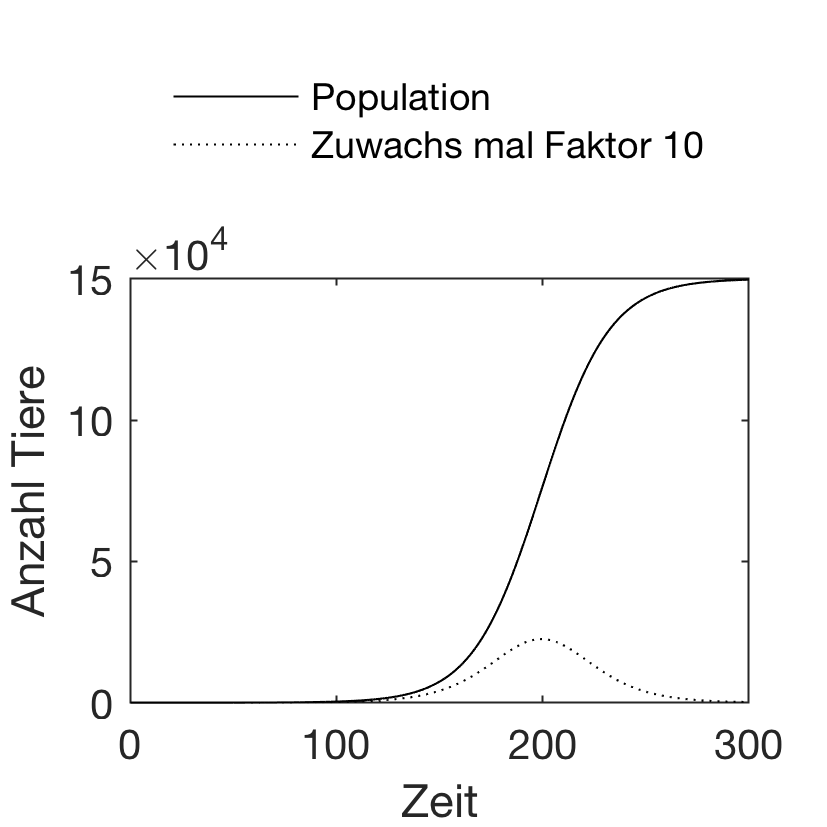
\includegraphics[width=5.5cm]{Diagramme/wachstum_ohne_einfluesse.png}
  		\caption{Population der Blauwale in der Antarktis.}
  		\label{fig:wachstum_ohne_einfluesse}
	\end{figure}

	Dabei bleibt die Population bei \(y = K\) im stabilen Gleichgewicht.

	Im nächsten Schritt wird die Gleichung durch einen äußeren Einfluss, die Fangintensität \(E\) erweitert:
	\begin{align*}
		%y(t+\Delta t) &= y(t) + r \cdot \left(1-\frac{y(t)}{K}\right) \cdot y(t) \cdot \Delta t - E \cdot y(t) \cdot \Delta t \\
		%&= \left(1+r \cdot \left(1-\frac{y(t)}{K}\right)\cdot \Delta t - E \cdot \Delta t \right) \cdot y(t)
		\dot{y} &= r \cdot\left(1-\frac{y}{K}\right) \cdot y - E \cdot y
	\end{align*}	
	
	\newpage	
	
	Anschließend wird die neue Gleichung in die Form der Anfangsgleichung gebracht:
		
	\begin{align*}
		%&= \left(1+r \cdot \left(\underbrace{1 - \frac{E}{r}}_{\textrm{ausklammern}} - \frac{y(t)}{K} \right) \cdot \Delta t \right) \cdot y(t) \\		
		%&= \left(1+\underbrace{r \cdot \left( 1 - \frac{E}{r} \right)}_{\tilde{r}} \cdot \left(1 - \frac{y(t)}{\underbrace{K \cdot \left( 1 - \frac{E}{r} \right)}_{\tilde{K}}} \right) \cdot \Delta t \right) \cdot y(t) \\		
		\dot{y} &= \left( r \cdot\left(1 - \frac{y}{K}\right) - E\right) \cdot y \\
		&= r \cdot \left( 1 - \frac{E}{r} - \frac{y}{K} \right) \cdot y \\
		&= \underbrace{r \cdot \left( 1 - \frac{E}{r} \right)}_{\tilde{r}} \cdot \left( 1 - \frac{y}{\underbrace{K \cdot \left(1 - \frac{E}{r}\right)}_{\tilde{K}}} \right) \cdot y
	\end{align*}
	
	Dabei beschreibt das \(\tilde{r}\) wiederum das proportionale Wachstum und \(\tilde{K}\) das Maximum der Populationsgröße. Den höchsten Ertrag erhält man, wenn sich die Population im stabilen Gleichgewichtspunkt \(y = \tilde{K} = K \cdot \left(1 - \frac{E}{r}\right) \) befindet. Somit wird der maximale Betrag durch \(E \cdot K \cdot \left(1 - \frac{E}{r}\right)\) beschrieben. Die Parameter \(r\) und \(K\) sind bekannt und um nun das maximale \(E\) zu finden, muss das Maximum der Funktion \(f(E) = E \cdot K \cdot \left(1 - E \cdot \frac{1}{r}\right)\) gesucht werden:
	\begin{align*}
		&f'(E) = K - 2 \cdot E \cdot \frac{K}{r} = K \left(1 - E \cdot \frac{2}{r} \right) \stackrel{!}{=} 0 \\
		&\Rightarrow 1 - E \cdot \frac{2}{r} = 0 \Rightarrow E = \frac{r}{2}
	\end{align*}
	Der maximale Ertrag ist somit gegeben durch:
	\begin{align*}
		\frac{r}{2} \cdot K \cdot \left(1 - \frac{r}{2}\cdot\frac{1}{r}\right) = \frac{r \cdot K}{4}
	\end{align*}
	
	Die nachfolgenden Abbildungen \ref{fig:zuwachs_etrag_auf_zeit1} und \ref{fig:zuwachs_etrag_auf_zeit2} zeigen den Zuwachs und den Ertrag über die Zeit für zwei unterschiedliche \(E\)'s.
	\begin{figure}[!h]
  		\centering
 		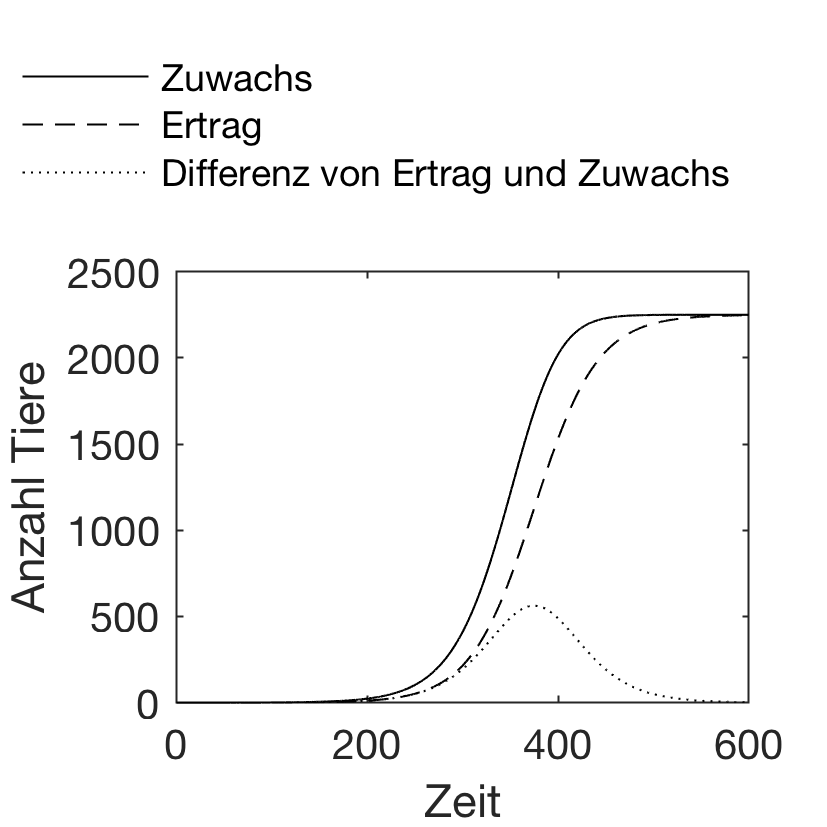
\includegraphics[width=5.5cm]{Diagramme/zuwachs_etrag_auf_zeit1.png}
  		\caption{Zuwachs und Ertrag für \(E = \frac{r}{2}\).}
  		\label{fig:zuwachs_etrag_auf_zeit1}
	\end{figure}
	\begin{figure}[!h]
  		\centering
 		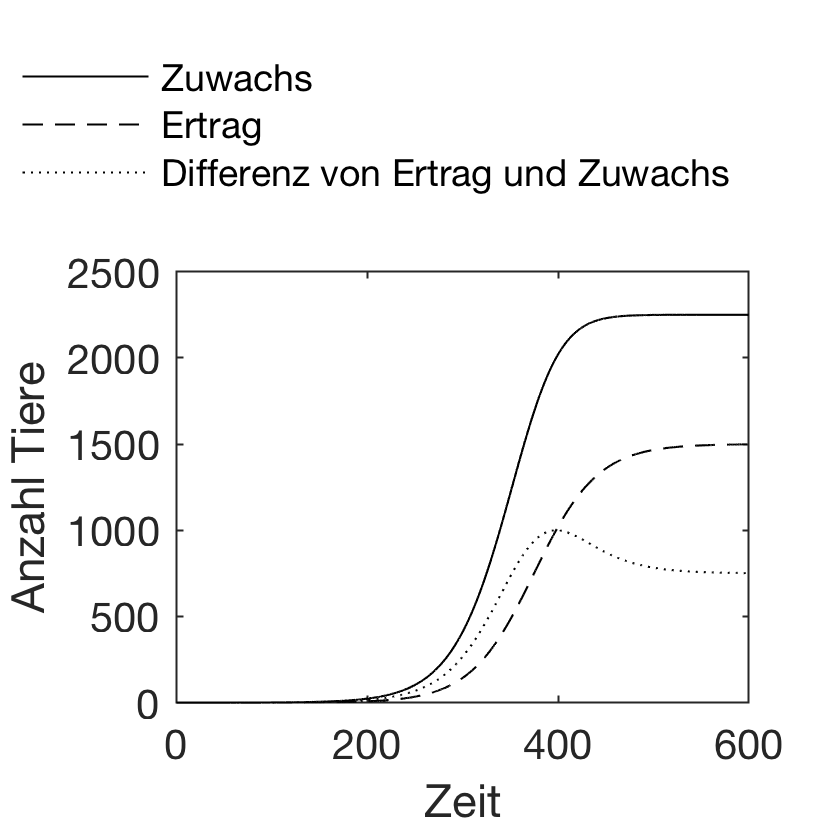
\includegraphics[width=5.5cm]{Diagramme/zuwachs_etrag_auf_zeit2.png}
  		\caption{Zuwachs und Ertrag für \(E = \frac{r}{3}\).}
  		\label{fig:zuwachs_etrag_auf_zeit2}
	\end{figure}

	Gut zu erkennen ist in Abbildung \ref{fig:zuwachs_etrag_auf_zeit1}, dass die Differenz von Ertrag und Zuwachs auf Null fällt sobald das Populationsmaximum erreicht ist. Dies geschieht in Abbildung \ref{fig:zuwachs_etrag_auf_zeit2} nicht. Es werden also nicht alle Wale gefangen und das Ertragsmaximum wird nicht erreicht.

	\newpage
	In Abbildung \ref{fig:zuwachs_ertrag_zu_population} ist dies ebenfalls zu erkennen, wenn der Zuwachs und Ertrag als Funktion der Populationsgröße aufzeichnet wird:
	\begin{figure}[!h]
  		\centering
 		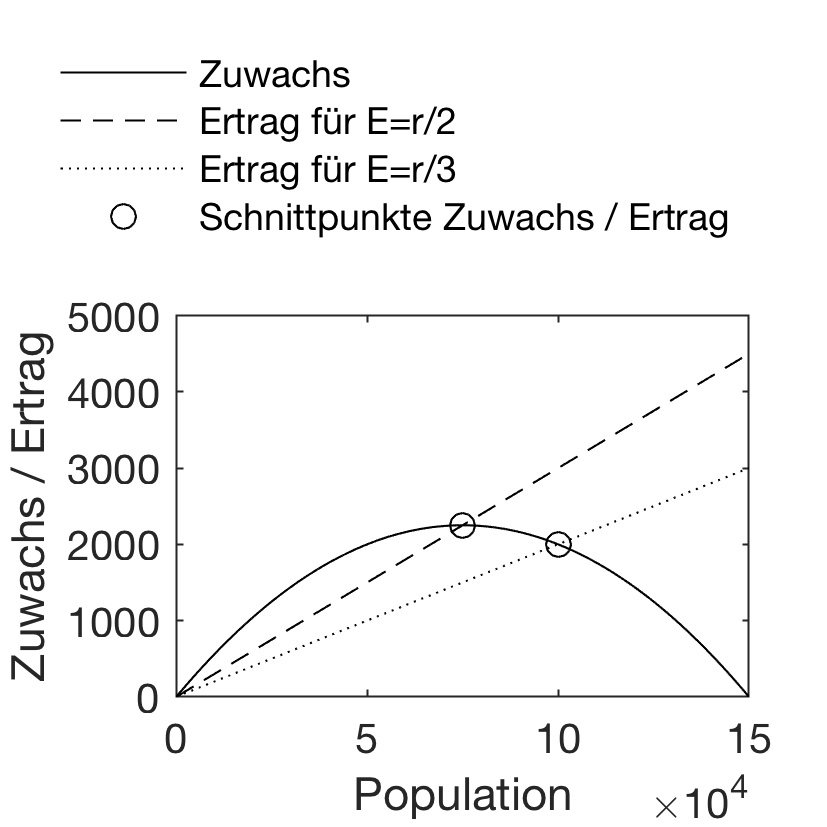
\includegraphics[width=5.5cm]{Diagramme/zuwachs_ertrag_zu_population.png}
  		\caption{Zuwachs (ohne äußere Einflüsse) und Ertrag als Funktion der Populationsgröße.}
  		\label{fig:zuwachs_ertrag_zu_population}
	\end{figure}

	Für \(E=\frac{r}{2}\) ist der Schnittpunkt zwischen Zuwachs und Ertrag genau im Maximum der Zuwachsfunktion. Für \(E=\frac{r}{3}\) hingegen leicht daneben, somit wird hierfür das Maximum nicht erreicht.
	
	\newpage
	
	\section{\uppercase{Räuber und Beute}}\label{sec:Raeuber_Beute}
	
	Zusätzlich zu den Walen wird eine weitere Spezies betrachtet, welche in Wechselwirkung mit den Walen steht, beispielsweise Plankton. Zur Vereinfachung werden im nachfolgenden Text die Population der Wale als Räuber \(w(t)\) und das Plankton als Beute \(v(t)\) bezeichnet. Die Population beider Arten verhält sich wie in Abschnitt \ref{sec:Wachstumsgleichung} beschrieben, wobei jedoch das Populationsmaximum jeweils von der Summe beider Arten abhängt:
	\begin{align*}
		\textrm{Räuber (Wale): } &\quad \dot{w} = -r_w \cdot \left(1 - \frac{w+v}{K} \right) \cdot w \\
		\textrm{Beute (Plankton): } &\quad \dot{v} = +r_v \cdot \left(1 - \frac{w+v}{K} \right) \cdot v
	\end{align*}

	Dabei beschreibt der Faktor \(r_v\) die Reproduktionsrate der Beute (positives Vorzeichen) und der Faktor \(r_w\) die Sterberate der Räuber (negatives Vorzeichen), denn diese verhungern falls sie kein Futter finden.

	Nun stehen diese zwei Arten miteinander in Wechselwirkung. Dabei beschreibt der Faktor \(\alpha\) die Wahrscheinlichkeit einer Begegnung. Dieser ist einzig von der Gestalt des Biotops anhängig und für beide Arten gleich. Zusätzlich beschreibt die Konstante \(l_{v}\) wie viele Beutetiere bei der Begegnung gefressen werden (negatives Vorzeichen) und die Konstante \(l_{w}\) wie stark sich die Räuber nach der Mahlzeit vermehren (positives Vorzeichen). Mit diesen zusätzlichen Variablen ergeben sich folgende Gleichungen:
	 \begin{align*}
		\dot{w} &= -r_w \cdot \left(1 - \frac{w+v}{K} \right) \cdot w + l_w \cdot \alpha \cdot w \cdot v \\
		\dot{v} &= +r_v \cdot \left(1 - \frac{w+v}{K} \right) \cdot v - l_v \cdot \alpha \cdot w \cdot v
	\end{align*}

	Werden diese zwei Gleichungen mit der allgemein bekannten Lotka-Volterra Gleichung \cite{PredatorPrey} Seite 3 verglichen, ist leicht zu erkennen, dass diese damit identisch sind.
	
	\newpage

	Wie man in Abbildung \ref{fig:beute_raeuber_oszillation} erkennen kann, ist mit entsprechenden Parametern ein Schwingungsverhalten zu beobachten. Wobei die Phasen der Schwingungen der beiden Arten jeweils verschoben sind.
	
	\begin{figure}[!h]
  		\centering
 		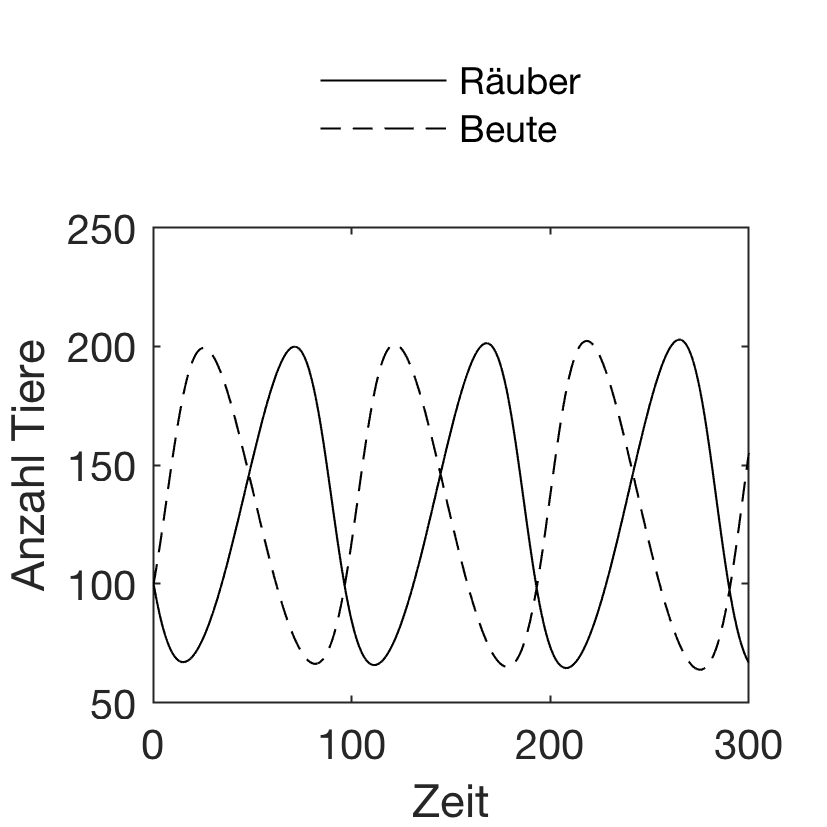
\includegraphics[width=5.5cm]{Diagramme/beute_raeuber_oszillation.png}
  		\caption{Population von Räuber und Beute als Funktion der Zeit mit \(r_w = r_v = l_v = l_w = 0.2; \alpha = 0.001\).}
  		\label{fig:beute_raeuber_oszillation}
	\end{figure}
	
	Um die Gleichgewichtspunkte der Gleichung für die Räuber zu untersuchen, setzen wir die Ableitung \(\dot{w}\) gleich null:
	\begin{align*}
		-r_w \cdot \left(1 - \frac{w+v}{K} \right) \cdot w + l_w \cdot \alpha \cdot w \cdot v &\stackrel{!}{=} 0\\
		-r_w \cdot \left(1 - \frac{w+v}{K} \right) + l_w \cdot \alpha \cdot v &= 0\\
		\frac{l_w \cdot \alpha \cdot v}{r_w} &= 1 - \frac{w}{K}-\frac{v}{K}\\
		\frac{K \cdot r_w - l_w \cdot \alpha \cdot w \cdot v - v \cdot r_w}{r_w} &= w
	\end{align*}
	
	Sei nun \(v=0\), so gilt für den Gleichgewichtspunkt der Räuber:
	\begin{align*}
		w = \frac{K \cdot r_w - l_w \cdot \alpha \cdot w \cdot 0 - 0 \cdot r_w}{r_w} = \frac{K \cdot r_w}{rw} = K
	\end{align*}	
	
	Somit bleibt die Population der Räuber bei \(w=K\) und \(v=0\) konstant. Dies entspricht aber keinesfalls der Realität, denn die Räuber können ja jeweils nur mit genügend Beute überleben. Dieses Beispiel zeigt somit eine theoretische Schwachstelle unseres Modells.
	
	\newpage
	
	\section{\uppercase{Agentenbasierte Modellierung}}
	
	In der agentenbasierten Modellierung werden Gleichungen im Gegensatz zur analytischen Modellierung mit einzelnen Individuen gelöst. Damit können zusätzlich real auftretende Effekte wie Überalterung oder ein Mindestalter zur Fortpflanzung berücksichtigt werden.
	
	Das agentenbasiertes Modell wurde speziell auf den Beute-Räuber Effekt angewendet, da dieser Effekt analytisch nur schwer zu lösen ist und Effekte wie Überalterung dort eine wichtige Rolle spielen. Die Individuen erhalten durch ihr Alter spezielle Eigenschaften:
	\begin{itemize}
		\item Hat das Individuum das maximale Alter überschritten, stirbt es. Es isst also nicht mehr und ist nicht in der Lage, sich fortzupflanzen. Die Anzahl der Tiere welche durch Überschreiten der Altersgrenze sterben, werden nachfolgend mit \(w_{zu~alt}\) bezeichnet.
		\item Ist das Individuum unter einem gewissen Alter, wird es bei der Fortpflanzung nicht berücksichtigt, es frisst aber die normale Menge.
		\item Jedes Individuum zwischen dem Mindestalter zur Fortpflanzung und dem maximalen Alter frisst (als Räuber) andere Tiere und ist in der Lage, sich fortzupflanzen. Die Anzahl dieser Tiere wird nachfolgend als \(w_{erw}\) oder \(v_{erw}\) bezeichnet.
	\end{itemize}
	
	Damit gilt für die Veränderung der Population der Räuber folgende Gleichung:
	\begin{align*}
		\dot{w} = -w_{zu~alt} + l_w \cdot \alpha \cdot w_{erw} \cdot v - \beta \cdot w
	\end{align*}
	Wobei die Proportionalitätskonstante \(\beta\) die Anzahl der Tiere beschreibt, welche durch natürliche Umwelteinflüsse sterben.

	Da auch die Beutetiere ein minimales Alter für die Fortpflanzung haben, muss die Gleichung aus Abschnitt \ref{sec:Raeuber_Beute} wie folgt geändert werden:
	\begin{align*}
		\dot{v} &= +r_v \cdot \left(1 - \frac{w+v}{K} \right) \cdot v_{erw} - l_v \cdot \alpha \cdot w_{erw} \cdot v
	\end{align*}
	
		Somit wird eine Tierart durch folgende Konstanten definiert:
	\begin{itemize}
	\item Maximales Alter: Überschreitet das individuelle Alter des Tieres diesen Wert, so stirbt es.
	\item Erwachsenenalter: Sobald das Tier diesen Alterswert erreicht hat, kann es sich fortpflanzen.
	\item \(l_w\) (nur Räuber): Reproduktionsrate nach einem Mahl.
	\item \(\beta\) (nur Räuber): Sterberate durch Umwelteinflüsse.
	\item \(r_v\) (nur Beute): Reproduktionsrate.
	\item \(l_v\) (nur Beute): Sterberate durch gefressen werden.
	\end{itemize}
	\subsection{Implementation}
	Die agentenbasierte Simulation wurde mit Python 3.6 umgesetzt. Die einzelnen Einheiten wurden dabei durch einen einzigen Gleitkommawert, welcher den Zeitpunkt ihrer Geburt angibt, in einem sortierten Array für jede Tierart repräsentiert. Alle Konstanten können in einem json-File angepasst werden und es können auch weitere Tierarten ohne zusätzlichen Programmieraufwand hinzugefügt werden. Die Ergebnisse der Simulation wurden als CSV-Datei abgespeichert und in Matlab visualisiert.
	
	In einer ersten Version waren alle Tiere noch in einem unsortierten Array und jedes Tier war Instanz einer extra entworfenen Klasse. Diese Methode war aber relativ langsam und  Berechnungen mit bis zu 100.000 Tieren über 3000 Zeitschritte dauerten etwa eine Stunde. Mit der Optimierung über ein sortiertes Array und Darstellung der Tiere als Gleitkommazahl konnte die Rechenzeit für die selben Werte auf 52s reduziert werden.
	
	\newpage	
	
	Die in Abschnitt \ref{sec:Ergebnis_Agent_Model} besprochenen Ergebnisse sind mittels folgendem durch Pseudocode beschriebenen Verhaltens entstanden:
	
	\begin{small}
	\begin{verbatim}
Für jeden Zeitschritt:
  Erhöhe die aktuelle Zeit um delta_t

  Für jede Tierart:
    Für alle Tiere bei denen die Differenz der
    aktuellen Zeit zum Geburtszeitpunkt größer
    als das maximale Alter der Tierart ist:
      Das Tier stirbt.

    w = Anzahl der Tiere der Tierart.
    w_erw = Anzahl Tiere bei denen die Differenz der
    aktuellen Zeit zum Geburtszeitpunkt größer
    als das Erwachsenenalter der Tierart ist.

    Ist die Tierart ein Räuber:
      v = Anzahl der Beutetiere.
      Anzahl gefressener Beutetiere = w*v*alpha*lv
      Für jedes Beutetier welches gefressen wird:
        Ein zufälliges Beutetier stirbt.
            
      delta_pop = lw*alpha*w_erw*v - beta*w.

    Ist die Tierart ein Beutetier:
      delta_pop = rv*(1-(Total aller Tiere/K))*w_erw.

    Ist delta_pop positiv:
      Für jedes neugeborene Tier:
        Ein neues Tier wird geboren und 
        die aktuelle Zeit als Geburtstermin 
        wird gespeichert.

    Ist die Veränderung in der
    Population negativ:
      Für jedes sterbende Tier:
        Ein zufälliges Tier stirbt.	
 		
	\end{verbatim}
	\end{small}
	
	Die verwendeten Rechenregeln sind nicht streng deterministisch. Die Auswahl der Tiere, die gefressen werden, erfolgt rein zufällig. Darum kann es, beim erneuten Ausführen der Simulation, zu minimal unterschiedlichen Ergebnissen führen.
	
	\subsection{Ergebnis}\label{sec:Ergebnis_Agent_Model}
	
	\begin{figure}[!h]
  		\centering
 		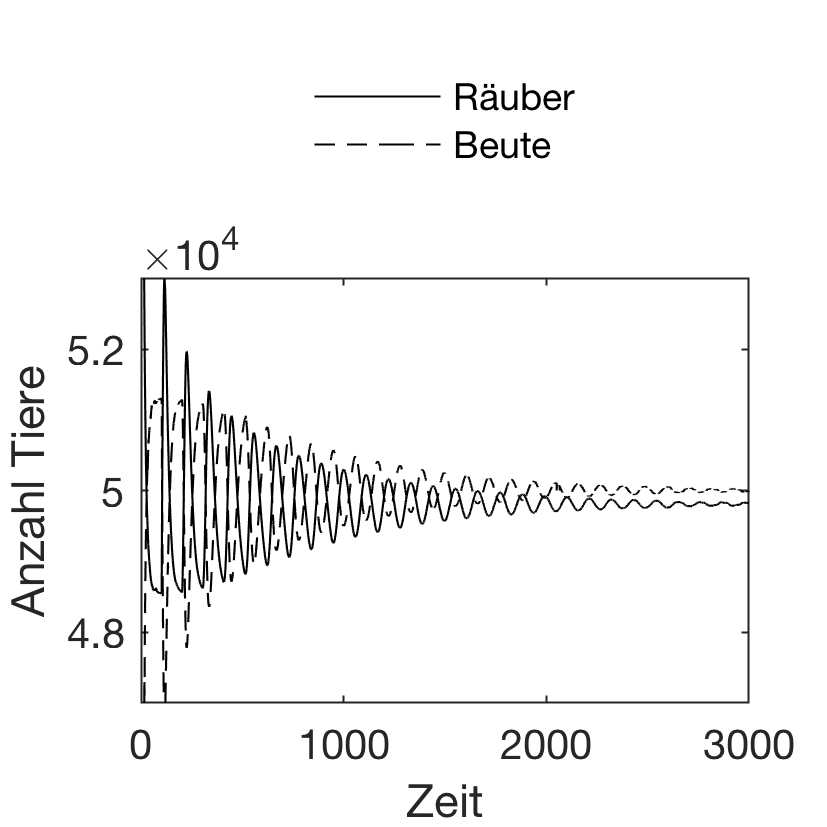
\includegraphics[width=5.5cm]{Diagramme/agent_model_damped.png}
  		\caption{Die Anzahl der Räuber und Beute Individuen in pendelt sich mittels gedämpfter Schwingung ein.}
  		\label{fig:agent_model_damped}
	\end{figure}
	
	In dem in Abbildung \ref{fig:agent_model_oscillation} dargestellten Diagramm sieht man eine ungebremste Schwingung. Diese tritt nur in sehr kleinen Wertebereichen auf. Meistens ist die Schwingung wie in Abbildung \ref{fig:agent_model_damped} gedämpft und pendelt sich auf einen festen Wert ein.
	
	\begin{figure}[!h]
  		\centering
 		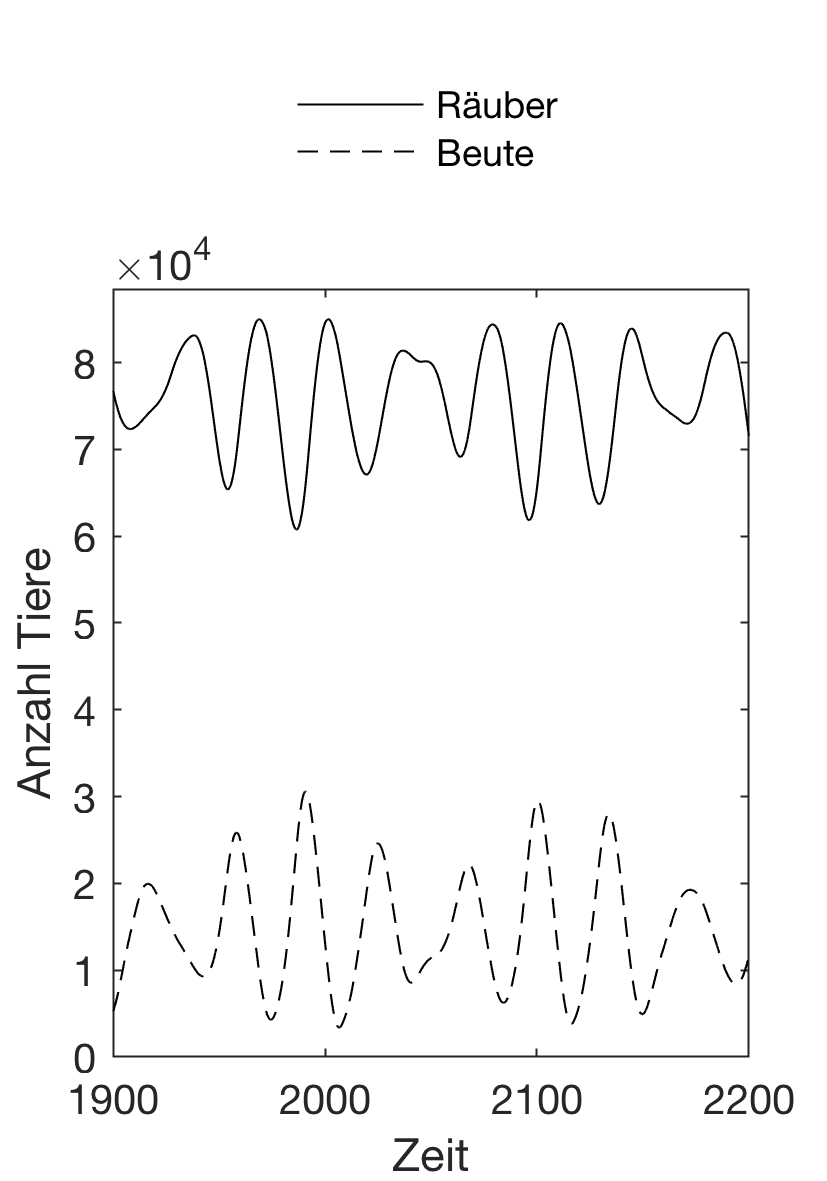
\includegraphics[width=5.5cm]{Diagramme/agent_model_oscillation.png}
  		\caption{Beispiel einer ungebremste Schwingung der Anzahl Räuber und Beute Individuen. Im dargestellten Ergebnis wurden 45\% der Beute aufgefressen und 55\% starben am Alter.}
  		\label{fig:agent_model_oscillation}
	\end{figure}
	
	Auffallend bei dem Diagramm ist, dass das maximale Alter der Räuber immer näherungsweise ein ganzzahliges Vielfaches der Periodendauer ist. Dies macht auch Sinn, da bei einem großen Anstieg der Bevölkerung viele Einheiten mit dem selben Alter entstehen. Diese Einheiten sterben also auch wieder gemeinsam, was eine Schwingung anregt. Da aber schon während des Sterbens mehr neue Einheiten erschaffen werden (und auch danach noch), ist diese Schwingung alleine betrachtet gedämpft.
	
	Eine weitere besondere Eigenschaft ist, dass bei Anfangswerten, die nicht zu weit vom Gleichgewicht entfernt sind und ohne Aussterben der Beute nie Jäger verhungert sind. 
	
	\subsection{Ausblick}
	Eine sinnvolle Erweiterung der Simulation wäre das Ausweiten auf mehrere Lebensräume. Der Aufbau der Simulation ist bereits darauf ausgelegt, einzig die Regeln für das Wandern zwischen den Lebensräumen müssten definiert und implementiert werden.
	
	\newpage	
	
	\section{\uppercase{Der zelluläre Automat}}
	
	Weiter wird untersucht, ob ein Schwingungsverhalten wie in Abschnitt \ref{sec:Raeuber_Beute} beschrieben, auch bei einem zellulären Automaten zu beobachten ist. Dafür wird ein WATOR System verwendet. Die hier verwendete Implementation ist der Beschreibung aus \cite{Wator} nachempfunden hat aber durchaus auch Ähnlichkeiten mit der Implementation aus \cite{PlanetWator}.	
	
	\subsection{Implementation}
	Nachfolgend wird auf die Einzelheiten der Implementation des zellulären Automaten eingegangen, dabei wird die Spezies der Räuber als Haie bezeichnet und die der Beutetiere als Fische.
	
	Als Datenstruktur des Automaten dient eine \(m \times m\) Matrix, wobei \(m\) die Größe des Lebensraums definiert. Diese \(m \times m\) Matrix hat wiederum drei Ebenen.
	
	Es existiert an der Stelle \(i,j\) der Matrix ein ...
	\begin{enumerate}[label=...]
		\item Fisch, falls der Wert \((i,j,1) > 0\) ist. Dieser Wert wird als Brutzeit der Fische bezeichnet.
		\item Hai, falls der Wert \((i,j,2) > 0\) ist. Dieser Wert wird als Brutzeit der Haie bezeichnet.
	\end{enumerate}
	Wobei an der Stelle \(i,j\) niemals ein Fisch und ein Hai gleichzeitig sein kann.

	Der Wert an der Stelle \((i,j,3)\) wird als zusätzliche Information für den Hai an der Stelle \(i,j\) benötigt und wird als Fastenzeit bezeichnet.

	Als angrenzende Felder der Stelle \(i,j\) sind die 4 Felder \((i+1,j), (i-1,j), (i,j+1), (i,j-1)\) definiert, wobei \( \forall i,j \in [1,m] \) gilt und bei Überlauf beziehungsweise Unterlauf wieder bei \(1\) beziehungsweise \(m\) weiter gezählt wird.
	
	Zusätzlich werden folgende Konstanten für die Simulation benötigt: \newline
	Reproduktionszeit der Fische: Sobald der Brutzeit-Wert eines Fisches unter diesen Wert fällt, wird ein neuer Fisch geboren. \newline
	Reproduktionszeit der Haie: Sobald der Brutzeit-Wert eines Haies unter diesen Wert fällt, wird ein neuer Hai geboren. \newline
	Überlebenszeit ohne Essen: Sobald der Fastenzeit-Wert eines Haies unter diesen Wert fällt, stirbt der Hai.
	
	Die Fische sowie die Haie werden jeweils in einem separaten Durchlauf berechnet. Es werden also zuerst alle Fische, danach alle Haie berechnet. Dabei ist die Rechenreihenfolge in jedem Durchlauf zufällig. Um Kollisionen zu vermeiden, werden jeweils alle neu berechneten Werte in eine neue Matrix geschrieben. Um nun leere angrenzende Felder zu finden, wird jeweils immer die alte sowie die neue Matrix betrachtet. So wird vermieden, dass sich ein Fisch oder Hai auf das gleiche Feld bewegen kann. Dieses Implementationsdetail unterscheidet sich von \cite{PlanetWator} wo alleine mit Wahrscheinlichkeiten gerechnet wird.
	
	
	\subsubsection{Das Verhalten der Fische}
	Jeder Fisch durchläuft folgendes durch Pseudocode beschriebenes Verhalten:

	\begin{small}
	\begin{verbatim}
Dezimiere den Brutzeit-Wert des Fisches.
 		
Falls ein leeres angrenzendes Feld existiert:
  Bewege auf zufälliges leeres Feld.
 			
  Falls der Brutzeit-Wert kleiner ist
  als die Reproduktionszeit für Fische:
    Ein neuer Fisch wird auf einem zufälligen
    leeren angrenzenden Feld geboren.
    Der Brutzeit-Wert wird auf einen neuen
    zufälligen Startwert zurückgesetzt.
 			
sonst:
  Bleibe stehen. 		
 		
	\end{verbatim}
	\end{small}
	
	\subsubsection{Das Verhalten der Haie}
	Jeder Hai durchläuft folgendes durch Pseudocode beschriebenes Verhalten:

	\begin{small}
	\begin{verbatim}
Dezimiere den Brutzeit-Wert des Haies.
		
Falls auf einem angrenzenden Feld
ein Fisch existiert:
  Gehe auf das Feld mit dem Fisch.
  Der Fisch auf diesem Feld stirbt.
  Der Fastenzeit-Wert wird auf einen neuen
  zufälligen Startwert zurückgesetzt.
		    
Falls ein leeres angrenzendes Feld existiert:
  Dezimiere den Fastenzeit-Wert.
  Falls der Fastenzeit-Wert kleiner ist als 
  die Überlebenszeit ohne Essen:
    So stirbt der Hai.
		        
  sonst:
    Gehe auf zufälliges leeres Feld.
		        
    Falls der Brutzeit-Wert kleiner ist
    als die Reproduktionszeit für Haie:
      Ein neuer Hai wird auf einem zufälligen
      leeren angrenzenden Feld geboren.
      Der Brutzeit-Wert wird auf einen neuen
      zufälligen Startwert zurückgesetzt.
		
sonst:
  Bleibe stehen. 
		
	\end{verbatim}
	\end{small}
	
	\newpage
	
	\subsection{Auswertung}
	Für die Simulation wurde eine \(128 \times 128\) Matrix verwendet. Als Ausgangslage wurden jeweils 128 Fische sowie 128 Haie an zufälliger Position mit zufälligem Brutzeit-Wert verwendet. In den ersten 500 Zyklen (siehe Abbildung \ref{fig:wator_diagram_100}) scheint das Verhalten noch recht zufällig:
	\begin{figure}[!h]
  		\centering
 		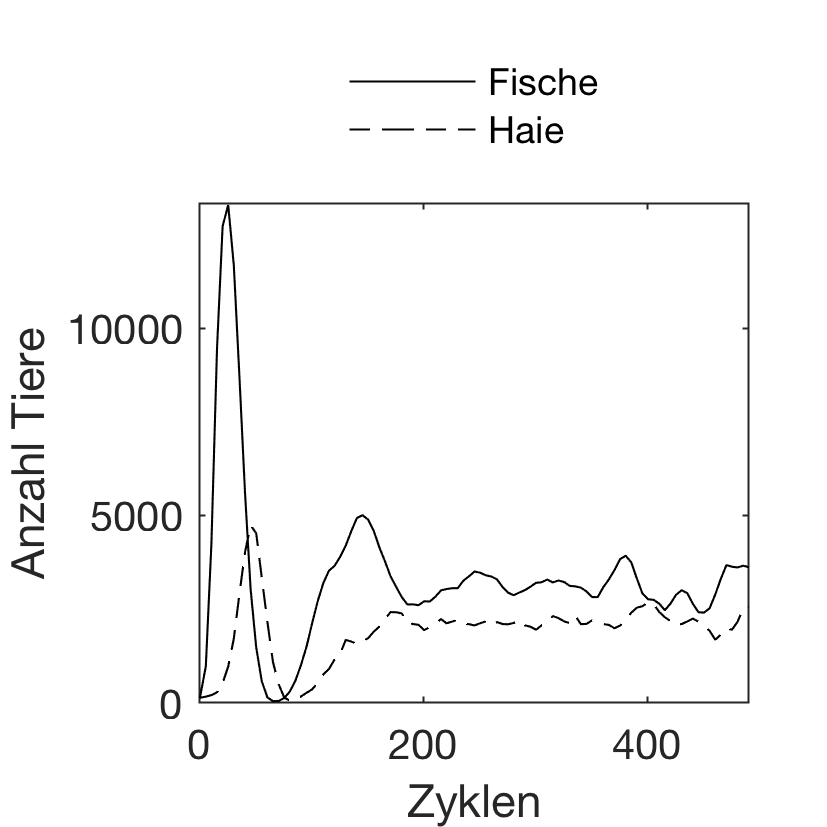
\includegraphics[width=5.5cm]{Diagramme/wator_diagram_100.png}
  		\caption{Die ersten 500 Zyklen der Wator-Simulation.}
  		\label{fig:wator_diagram_100}
	\end{figure}
	
	\begin{figure}[!h]
  		\centering
 		
\includegraphics[width=5.5cm]{Diagramme/wator_image_100.png}
  		\caption{Die Wator-Simulation nach 500 Zyklen: Der Brutzeit-Wert der Fische ist als Graustufenskala von Weiss (Maximum) bis Grau (Minimum) dargestellt. Der Fastenzeit-Wert der Haie ist als Graustufenskala von Schwarz (Maximum) bis Grau (Minimum) dargestellt. }
  		\label{fig:wator_image_100}
	\end{figure}
	
	Wie in Abbildung \ref{fig:wator_image_100} zu erkennen ist, sind die Fisch sowie die Hai Ansammlungen der Simulation jedoch nicht mehr völlig zufällig. Es bilden sich immer mehr Fisch- und Hai-Fronten, welche sich als Gruppe fortbewegen. Tatsächlich bildet sich auch nach weiteren 1000 Zyklen ein deutliches Schwingungsverhalten ab, wie die Abbildung \ref{fig:wator_diagram_348} zeigt.
	\begin{figure}[!h]
  		\centering
 		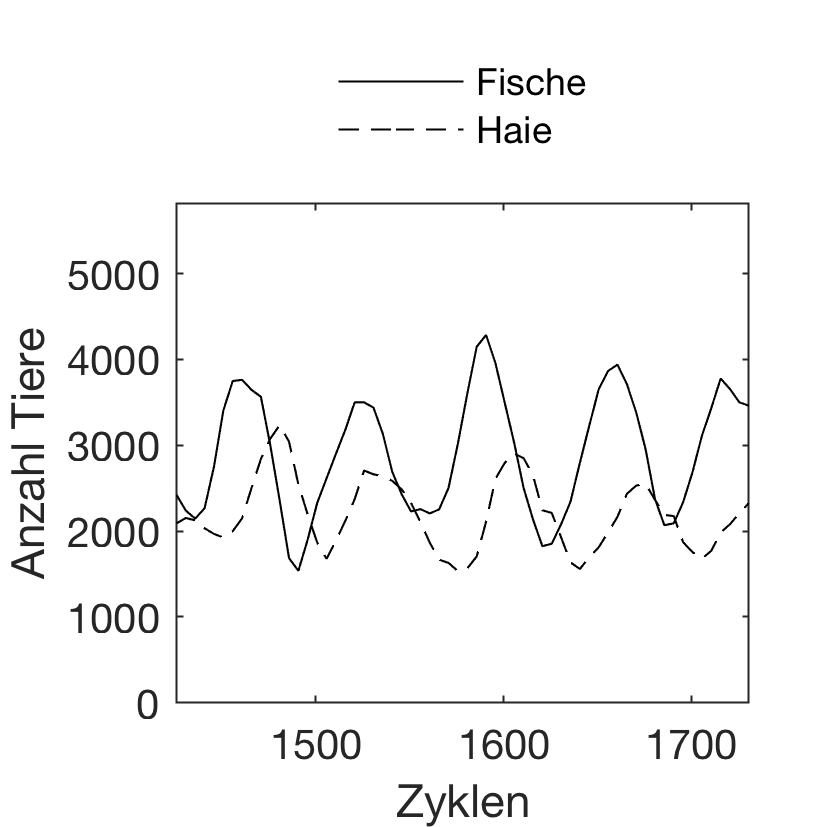
\includegraphics[width=5.5cm]{Diagramme/wator_diagram_348.png}
  		\caption{Schwingungsverhalten nach weiteren 1000 Zyklen.}
  		\label{fig:wator_diagram_348}
	\end{figure}

	\newpage

	\subsection{Fazit}
	Das Modell zeigt Schwingungsverhalten. Wobei aber kleinste Änderungen der Konstanten sowie der Anfangswerte großen Einfluss auf das Ergebnis haben. Ein gleichmäßiges Schwingungsverhalten zeigt sich jeweils nur durch geschicktes Wählen der Variablen. Dabei können die gleichen Konstanten für eine größere oder kleinere Matrix nicht mehr funktionieren, somit ist also die Größe der Umgebung durchaus maßgeblich für ein stabiles Gleichgewicht der beiden Spezies.
	
	In den beschriebenen Versuchen wurde bisher nur gezeigt, dass die Wator-Simulation durchaus ein ähnliches Verhalten zeigt wie das klassische Räuber-Beute Modell oder das agentenbasierte Modell. Wobei sich aber bei einer leeren Umgebung keine weiteren Vorteile zeigen. Dies würde sich ändern sobald nicht mehr nur eine leere Umgebung betrachtet wird. So könnten zum Beispiel räumliche Grenzen wie Inseln oder Wasserstraßen miteinbezogen werden.
	
	\newpage
	
	\vfill
	\bibliographystyle{apalike}
	{\small
	\bibliography{literatur}}
	
	\section*{Quellcode}
	Der gesamte Quellcode der beschrieben Simulationen ist unter https://git.io/vNc4o offen zugänglich.

\end{document}	

